% Donna Mustafa
For the purpose of our study, SolidWorks was used as a CAD software, as it contains solid modelling, Motion studies, Simulation PhotoView 360, e-drawing and many other features that were used to obtain a complete CAD model for KR6 r900 sixx KUKA arm. 
\newline In Simulation and Analysis, you can test your designed product in real environment.In simulation process the model can be tested against parameters like static and dynamic response, fluid dynamic, heat transfer. It also supports thermal, fatigue, structural and motion analysis. 
\newline In our project, SolidWorks is used to obtain a CAD model for KR6 r900 sixx and to perform a motion analysis study on the model. In addition to designing a base to fix the robot arm, perform a stress analysis and creating an animation video of the model’s motion.

\subsection{Complete CAD model}

\subsubsection{Searching for a suitable model}
All CAD models for KR6 r900 sixx on KUKA website or GrabCAD were step imported parts which are treated as a one body where joints can’t rotate therefore, motion study can’t be performed because it was impossible to add motors at the robot joints. The solution for this issue was obtained by converting step parts into assembly, which is done through several steps:
\begin{itemize}
	\item Open the .stp file part in SOLIDWORKS.  Select the file type to be .stp
	\item Click the OPTIONS tab, select Import multiple bodies as parts and click OK.
	\item Then click Open.
\end{itemize}
SolidWorks will create an assembly and create an individual part file for each multibody (Part1,Part2,Part3 etc.)
\begin{figure}[h]
	\centering
	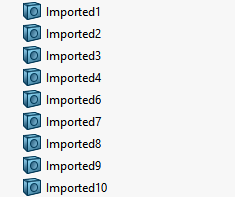
\includegraphics{figures/Stepparts}
   \caption{Step parts}
\end{figure}
\begin{figure}[h]
	\centering
	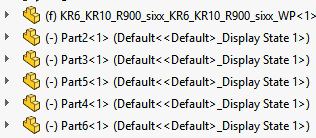
\includegraphics{figures/assemblyparts}
    \caption{SolidWorks parts}
\end{figure}

\subsubsection{Modifications on CAD model}
 \paragraph{Material and weights}
 The robot material wasn’t specified and the model was a whole body, and the total mass for the robot was 33.74 Kg, which was not accurate, because the actual mass of the robot, according to the KR6 R900 sixx dimensions manual, must be approximately equal to 52Kg. This is achieved by making the model hollow, using the shell feature and adding to joins point masses similar to the real motors with mass approximate equal to motors masses. 
\begin{figure}[h]
	\centering
	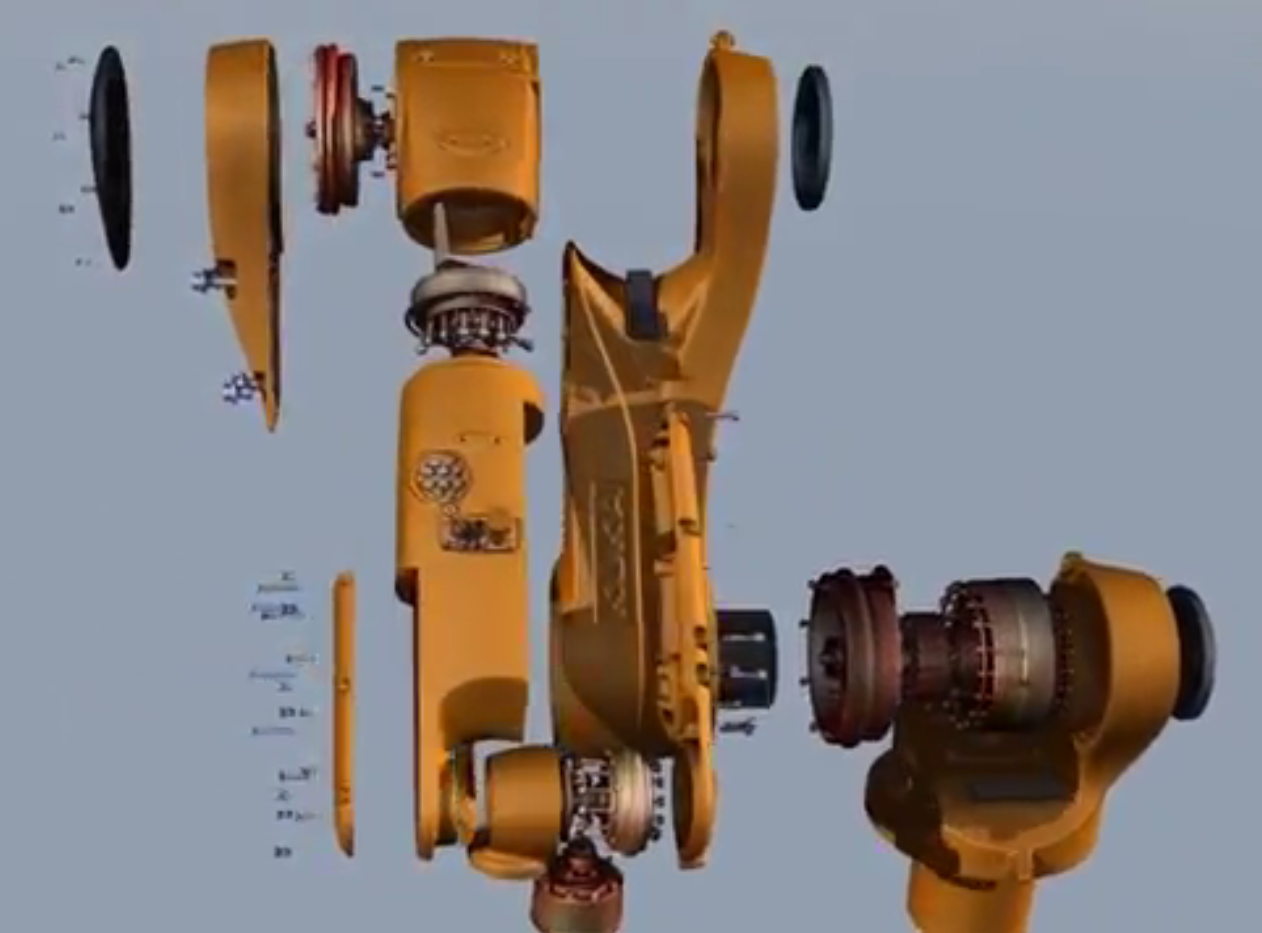
\includegraphics[scale=0.5]{figures/KUKAmotor}
    	\caption{KUKA motors}
\end{figure}

\begin{figure}
    \centering
    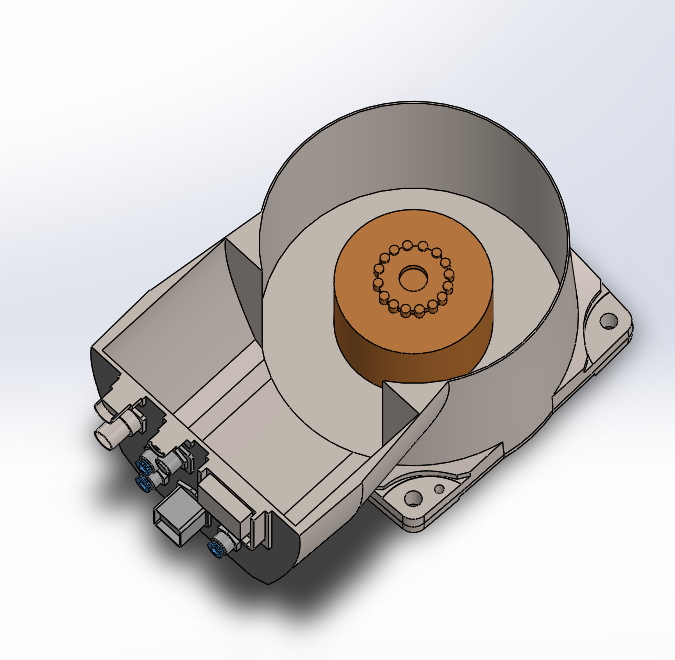
\includegraphics[width=0.45\linewidth]{Motor1}
    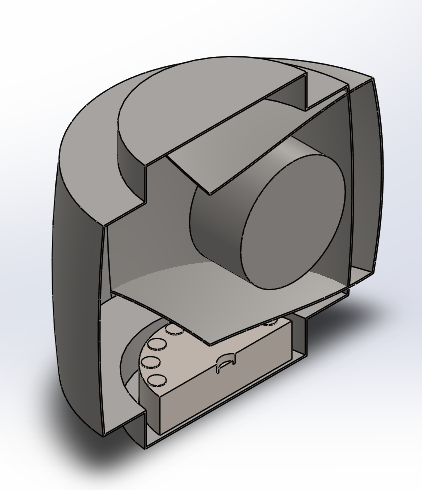
\includegraphics[width=0.45\linewidth]{Motor3}
    \caption{Motors  1,2 and 3 , 4,5 and 6 models}
    \label{fig:motorModels}
\end{figure}

\begin{figure}
	\centering
	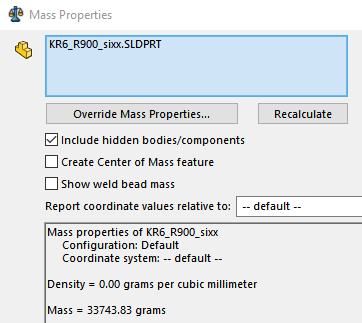
\includegraphics[width=0.45\linewidth]{Massbeforeadjust}
	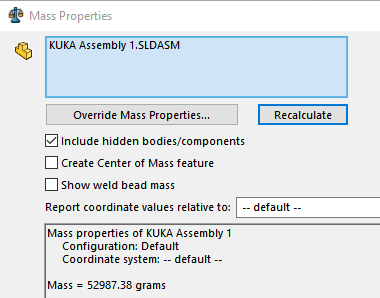
\includegraphics[width=0.45\linewidth]{Finalmass}
	\caption{The model mass: Old mass and final mass}
	\label{fig:sfig2}
\end{figure}
 
\paragraph{Spindle}
In order to have a complete model for our graduation project, a router spindle and its holder were sketched to complete the existing KUKA model.
\begin{figure}[h]
	\centering
	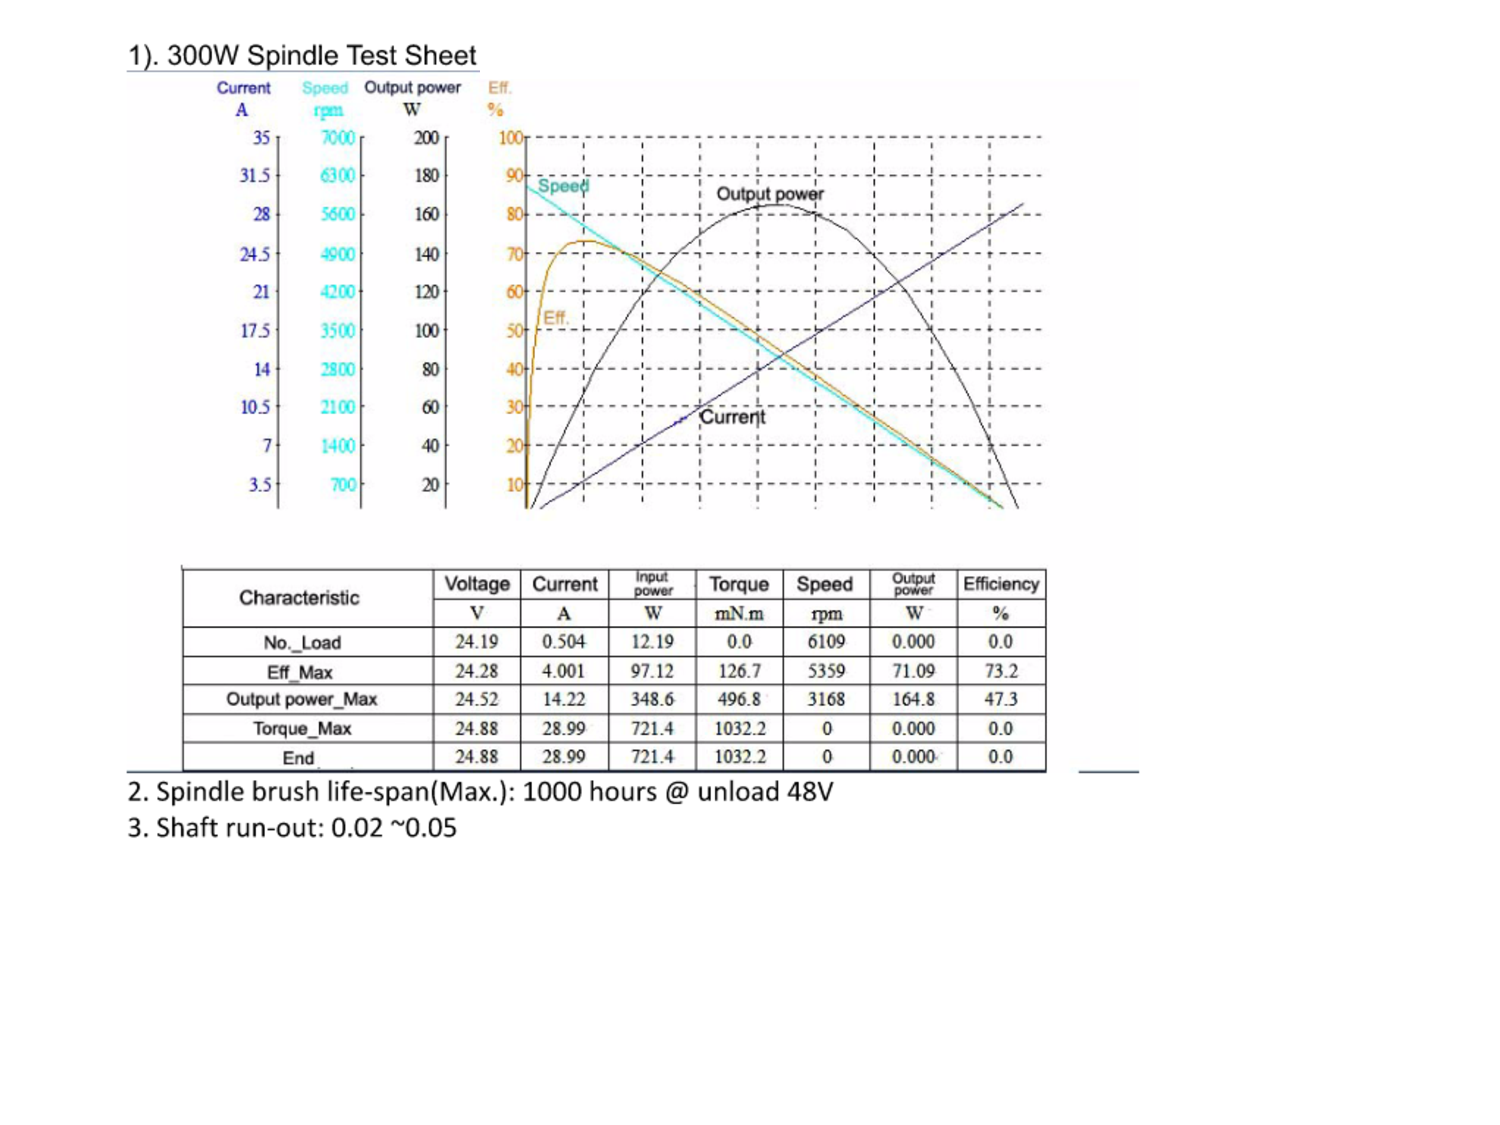
\includegraphics[scale=0.4]{spindle}
    	\caption{Spindle model}
\end{figure}

\begin{figure}[h]
	\centering
	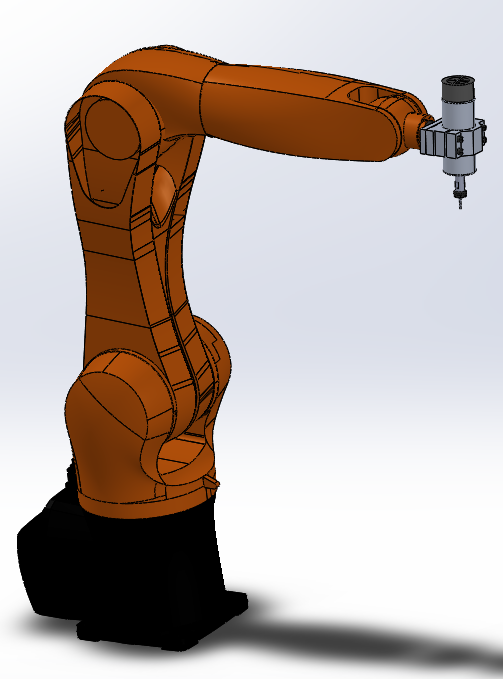
\includegraphics[scale=0.7]{FinalCADmodel}
    	\caption{Final CAD model}
\end{figure}

\newpage
\subsection{Motion studies}
Motion studies are graphical simulations of motion for assembly models. They simulate and animate the prescribed motion for a model. SolidWorks offer three different types of motion study, Animation, Basic Motion and Motion Analysis. They also offer mate controller that show, save the positions of assembly components at various mate values and degrees of freedom and create simple animations between those positions.

 Animation can be used to animate the motion of assembly. If you simply wish to create some nice visuals for presentation or marketing without consideration of mass and gravity effects, then animation is for you. 

 Basic Motion is an extra layer of complexity that takes into consideration the effects of mass, motors, springs, contact, and gravity on assemblies. 

 Motion Analysis is the top tier of motion study provides accurately simulation and analyze the motion of an assembly while incorporating the effects of Motion Study elements (including forces, springs, dampers, and friction). Motion Analysis can also be used to plot simulation results for further analysis.

 Therefore, Motion Analysis is used to simulate the model, generating results and plots of the simulation and Animation is used to make a video for motion.

\subsubsection{Animation study} 
 Animation study is done to make an animation video of the moving parts with the use of limit mates. Limit angle mate is an advanced mate type that is performed by selecting two planes which rotate with respect to each other giving the desired range to mate and input a maximum and minimum value for the angle to specify the desired range of motion. Another advantage of limit angle is that it prevent collision between the moving parts.
\begin{figure}[h]
	\centering
	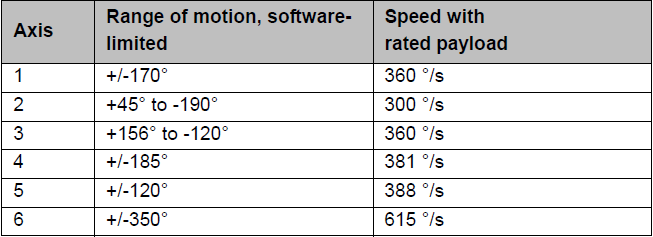
\includegraphics[scale=0.7]{Axesrangeofmotion}
    	\caption{Axes range of motion}
\end{figure}

\newpage
\subsubsection{Motion analysis}
 On implementing motion analysis by adding a motor at the required location to start simulating the robot, a problem arose; the model exploded on running the simulation where some of the parts were separated from each other. This happened because of redundancy constrains. For Motion Analysis studies, having redundant mates is the equivalent of over-defining the model.  

\begin{figure}[H]
	\centering
	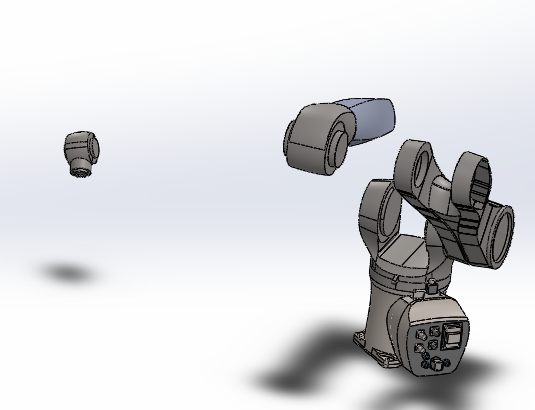
\includegraphics[scale=0.8]{Redundancyproblem}
    	\caption{Redundancy constraint problem}
\end{figure}

 This issue was solved by using mechanical mates of hinge type instead of standard mates. Hinge mate limits the movement between two components to one rotational degree of freedom. It has the same effect as adding a concentric mate plus a coincident mate and also limit the angular movement between the two components by adding limit angles. Reducing the negative effect of redundant mates on analysis.
\begin{figure}
	\centering
	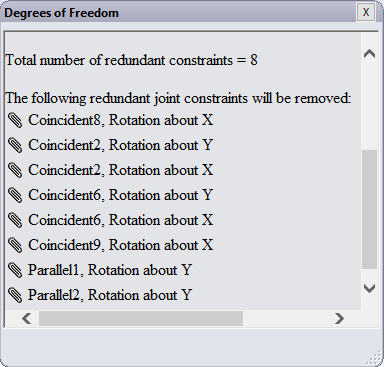
\includegraphics[scale=0.75]{redundancyconstrains}
    	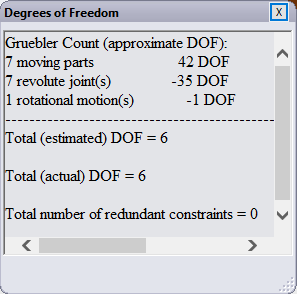
\includegraphics[scale=0.8]{zeroredandantcontraints}
    	\caption{present of redundancy constrains and Zero redundant constraints}
\end{figure}

 Now motors can be added to the model to perform any motion and results as motor torque, velocity, acceleration and force are generated.
 
\paragraph{Results of motion analysis study}] 
By assigning a motor to simulate the motion of axis and plotting the results to achieve this motion we found:
\begin{itemize}
	\item Results of motor torque for axis 1 to move 100 degrees in 4 seconds:
	\begin{figure}[H]
		\centering
		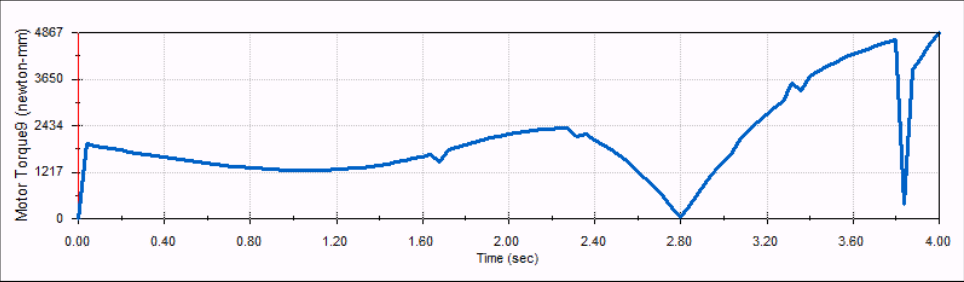
\includegraphics[width=\textwidth]{Motor1torque}
        \caption{Motor 1 torque}
	\end{figure}
Knowing that the actual motor torque for axis 1 is 4.5 N.m so the motion analysis result is approximate to actual torque. 
 
Motor torque vary with time because of the motion of the links beyond the motor which has an effect on the torque by changing the loads carried by the motor.
\item Motor 2 torque to move 60 degrees in 2 seconds:
	\begin{figure}[H]
    \centering
    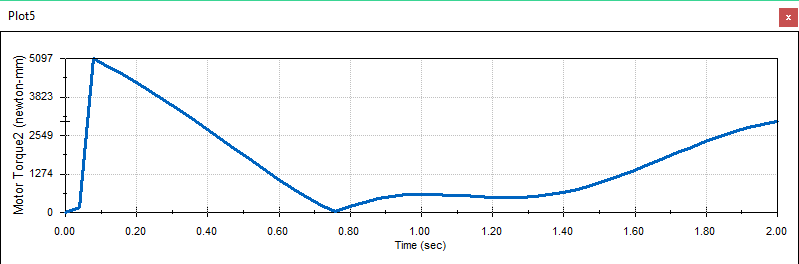
\includegraphics[width=\textwidth]{Motor2torque}
    \caption{Motor 2 torque}
\end{figure}
 Where the actual motor torque is 4 N.m

\item Motor torque for axis 3 to move 75 degrees in 1.8 seconds:
	\begin{figure}[H]
    \centering
    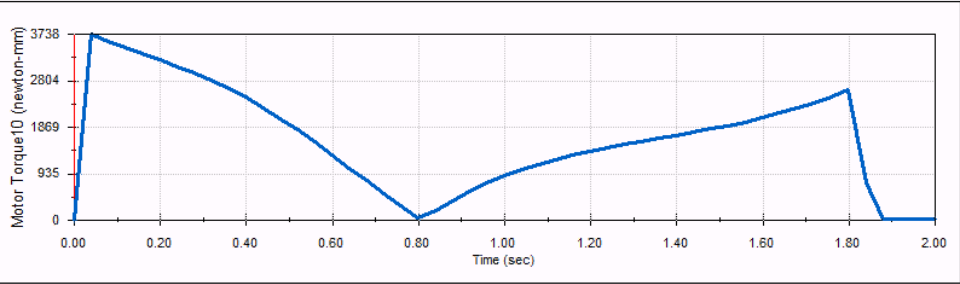
\includegraphics[width=\textwidth]{Motor3torque}
    \caption{Motor 3 torque}
\end{figure}

 Knowing that the actual motor torque for axis 3 is 3.5 N.m so the motion analysis result is approximate to actual torque.
\end{itemize}

\paragraph{Trace path}
Motion analysis results and plots have a trace path option that can trace the path of a point in the assembly. The selected point is end mill vertex to create the curve feature that represent the motion of the links.  By assigning a data point motors to the joints whose data is imported from excel spreadsheet of file type .csv containing two columns, first represent time in seconds while other is degrees of rotation. The generated curve of adding this data to joints 1-5 is an arc shape.
\begin{figure}[h]
	\centering
	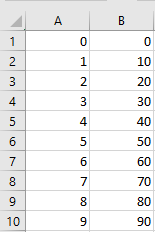
\includegraphics[scale=0.8]{datapoint}
    	\caption{Used data point}
\end{figure}
\begin{figure}[H]
	\centering
	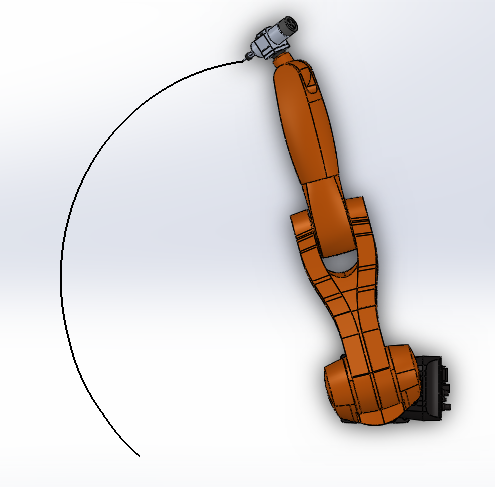
\includegraphics[scale=0.8]{Tracepathcurve}
    	\caption{Created curve}
\end{figure}

\section{Refrences}
\begin{itemize}
	\item \url{http://www.engineersrule.com/motion-studies-and-how-to-do-them}
	\item SolidWorks help
	\item SolidWorks forums
	\item Specification manual
	\item Dimensions manual
	\item \url{https://robotics.stackexchange.com/questions/10256/dynamic-torque-simulation-for-a-6-dof-robotic-arm}
\end{itemize}